% CSCI3753 - Operating Systems
% Spring 2014
% Programming Assignment 2
% Updated by Mike Gartrell (1/30/2014)

\documentclass[12pt]{article}

\usepackage[text={6.5in, 9in}, centering]{geometry}
\usepackage{graphicx}
\usepackage{url}

\title{Programming Assignment 2:\\DNS Name Resolution Engine}
\author{
  CSCI 3753 - Operating Systems\\
  University of Colorado at Boulder\\
  Due Date:  Friday, Feburary 21, 2014 11:55pm
}
\date{Spring 2014}

\begin{document}

\maketitle

\section{Introduction}
In this assignment you will develop a multi-threaded
application that resolves domain names to IP addresses, similar to the
operation preformed each time you access a new website in your web browser.
The application is composed of two sub-systems, each with one thread pool:
requesters and resolvers. The sub-systems
communicate with each other using a bounded queue.

This type of system architecture is referred to as a Producer-Consumer
architecture. It is also used in search engine
systems, like Google. In these systems, a set of crawler threads place
URLs onto a queue. This queue is then serviced by a set of indexer
threads which connect to the websites, parse the content, and then add
an entry to a search index. Refer to Figure \ref{fig:sys} for a
visual description.

\begin{figure}[htbp]
  \begin{center}
    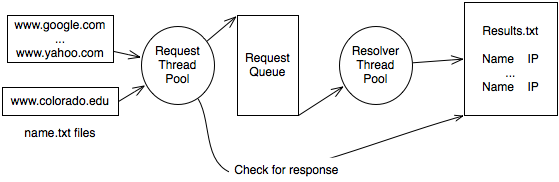
\includegraphics[width=100mm]{pa2.png}
    \caption{System Architecture}
    \label{fig:sys}
  \end{center}
\end{figure}

\section{Description}
\subsection{Name Files}
Your application will take as input a set of name files. Names files
contain one hostname per line. Each name file should be serviced by a
single requester thread from the requester thread pool.

\subsection{Requester Threads}
The requester thread pool
services a set of name files, each of which contains a list of domain
names. Each name that is
read from each of the files is placed on a FIFO queue.
If a thread tries to write to the
queue but finds that it is full, it should sleep for a random period
of time between 0 and 100 microseconds.

\subsection{Resolver Threads}
The second thread pool is comprised of a set of \texttt{THREAD\_MAX}
resolver threads. The
resolver thread pool services the FIFO queue by taking a name off the
queue and querying its IP address. After the
name has been mapped to an IP address,
the output is written to a line in the results.txt file in the
following format:

\begin{verbatim}
www.google.com,74.125.224.81
\end{verbatim}

\subsection{Synchronization and Deadlock}
Your application should synchronize access to shared resources and
avoid deadlock. You should use mutexes and/or semaphores to meet this
requirement. There are at least two shared resources that must be
protected: the queue and the output file. Neither of these resources
is thread-safe by default.

\subsection{Ending the Program}
Your program must end after all the names in each file have been
serviced by the application. This means that all the hostnames in all
the input files have received a corresponding line in the output file.

\section{What's Included}
Some files are included with this assignment for your benefit. You are
not required to use these files, but they may prove helpful.
\begin{enumerate}
\item {\bf queue.h} and {\bf queue.c} These two files implement the
  FIFO queue data structure. The queue accepts pointers to arbitrary
  types. You should probably use the queue to store pointers to
  C-strings of hostnames. The requester threads should push these
  hostnames into the
  queue, and the resolver threads should obtain hostnames from the same
  queue.

  Please consult the \textit{queue.h} header file for more detailed
  descriptions of each available function.

\item {\bf queueTest.c} This program runs a series of tests to confirm
  that the queue is working correctly. You may use it as an example of
  how to use the queue, or to test the functionality of the queue code
  that you are provided.

\item {\bf util.c} and {\bf util.h} These two files contain the DNS lookup
  utility function. This function abstracts away a lot of the
  complexity involved with performing a DNS lookup. The function
  accepts a hostname as input and generates a corresponding
  dot-formatted IPv4 IP address string as output.
  
  Please consult the \textit{util.h} header file for more detailed
  descriptions of each available function.
  
\item {\bf input/names*.txt} This is a set of sample name files.
  They follow the same format as mentioned earlier. Use them to test
  your program.

\item {\bf results-ref.txt} This result file is a sample output of the IPs
  for the hostnames from the \textit{names*.txt} files.

\item {\bf lookup.c} This program represents an un-threaded solution to
  this assignment. Feel free to use it as a starting point for your
  program, or as a reference for using the utility functions and
  performing file i/o in C.

\item {\bf pthread-hello.c} A simple threaded ``Hello World'' program
  to demonstrate basic use of the pthread library.

\item {\bf Makefile} A GNU Make makefile to build all the code listed
  here.

\end{enumerate}

\section{Additional Specifications}

Many of the specifications for your program are embedded in the
descriptions above. This section details additional specifications to
which you must adhere.

\subsection{Program Arguments}
Your executable program should be named ``multi-lookup''.
When called, it should interpret the last argument as the file path
for the file to which results will be written. All proceeding
arguments should be interpreted as input files containing hostnames in
the aforementioned format.

An example call involving three input files might look like:

\begin{verbatim}
multi-lookup names1.txt names2.txt names3.txt result.txt
\end{verbatim}

\subsection{Limits}
If necessary, you may impose the following limits on your
program. If the user specifies input that would require the violation
of an imposed limit, your program should gracefully alert the user to
the limit and exit with an error.

\begin{itemize}
\item {\bf MAX\_INPUT\_FILES}: 10 Files (This is an optional
  upper-limit. Your program may also handle more files, or an
  unbounded number of files, but may not be limited to less than
  10 input files.)
\item {\bf MAX\_RESOLVER\_THREADS}: 10 Threads (This is an optional
  upper-limit. Your program may also handle more threads, or match
  the number of threads to the number of processor cores.)
\item {\bf MIN\_RESOLVER\_THREADS}: 2 Threads (This is a mandatory
  lower-limit. Your program may handle more threads, or match
  the number of threads to the number of processor cores, but must
  always provide at least 2 resolver threads.)
\item {\bf MAX\_NAME\_LENGTH}: 1025 Characters, including null
  terminator (This is an optional upper-limit. Your program may handle
  longer names, but you may not limit the name length to less than
  1025 characters.)
\item {\bf MAX\_IP\_LENGTH}: INET6\_ADDRSTRLEN (This is an optional
  upper-limit. Your program may handle longer IP address strings, but
  you may not limit the name length to less than INET6\_ADDRSTRLEN
  characters including the null terminator.) 
\end{itemize}

\subsection{Error Handling}
You must handle the following errors in the following manners:

\begin{itemize}
\item {\bf Bogus Hostname}: Given a hostname that can not be resolved,
  your program should output a blank string for the IP address, such
  that the output file contines the hostname, followed by a comma,
  followed by a line return. You should also print a message to stderr
  alerting the user to the bogus hostname.
\item {\bf Bogus Output File Path}: Given a bad output file path, your
  program should exit and print an appropriate error to stderr.
\item {\bf Bogus Input File Path}: Given a bad input file path, your
  program should print an appropriate error to stderr and move on to
  the next file.
\end{itemize}

All system and library calls should be checked for errors.
If you encounter
errors not listed above, you should print an appropriate message to
stderr, and then either exit or continue, depending upon whether or not
you can recover from the error gracefully.

\section{External Resources}
You may use the following libraries and code to complete this
assignment, as well as anything you have written for this assignment:

\begin{itemize}
  \item Any functions listed in util.h
  \item Any functions listed in queue.h
  \item Any functions in the C Standard Library
  \item Standard Linux pthread functions  
  \item Standard Linux Random Number Generator functions
  \item Standard Linux file i/o functions
\end{itemize}

If you would like to use additional external libraries, you must clear
it with the TAs first. You will not be allowed to use pre-existing
thread-safe queue or file i/o libraries since the point of this
assignment is to teach you how to make non-thread-safe resources
thread-safe.

\section{What You Must Provide}
To receive full credit, you must submit the following items to Moodle
by the due date. Please combine the files into a single zip or tar
archive.

\begin{itemize}
\item {\bf multi-lookup.c}: Your program, conforming to the above
  requirements
\item {\bf multi-lookup.h}: A header file containing prototypes for any
  function you write as part of your program.
\item {\bf Makefile}: A makefile that builds your program as the
  default target. It should also contain a 'clean' target that will
  remove any files generated during the course of building and/or
  running your program.
\item {\bf README}: A readme describing how to build and run your
  program.
\item Any additional files necessary to build or run your program
\end{itemize}

\section{Extra Credit}

There are a few options for receiving extra credit on this
assignment. Completion of each of the following items will gain you 5
points of extra credit per item. In no case will the maximum score on
this assignment exceed 110/100.

\begin{itemize}
\item {\bf Multiple IP Addresses}: Many hostnames return more than a
  single IP address. Add support for listing an arbitrary number of
  addresses to your program. These addresses should be printed to the
  output file as additional comma-separated strings after the
  hostname. For example:
\begin{verbatim}
www.google.com,74.125.224.81,76.125.232.80,75.125.211.70
\end{verbatim}
You may find it necessary to modify code in the util.h and util.c
files to add this functionality. If you do this, please maintain
backwards compatibility with the existing util.h functions. This is
most easily done by adding new function instead of modifying the
existing ones.
\item {\bf IPv6 Support and Testing}: Add support for IPv6 IP
  addresses and find an IPv6 aware environment where you can test this
  support. Since IPv6 is relatively new, finding an environment
  for testing this support is probably harder than adding it. You must
  be able to demonstrate IPv6 support during your grading session to receive
  credit for this item. You may find it necessary to modify code in
  util.h and util.c to complete this item. If you do so, please
  maintain backward compatibility with the existing code.
\item {\bf Matching Number of Threads to Number of Cores}:
  Make your program dynamically detect the number of cores available on a
  system and set the number of resolver threads to take into account
  the number of cores.
\item {\bf Full-Loop Lookups}: Make each requester thread query the
  output file every 250ms to detect when each of its requests have
  been filled. Requester threads should print a message to the user
  with the IP address of each hostname, and should not exit until all
  of each threads requests have been satisfied.
\item {\bf Benchmarks}: Determine the ideal number of resolver threads
  for a given processor core count. Provide benchmark data backing up
  your determination. Include this documentation in your README.
\end{itemize}

\section{Grading}

Like all CS3753 assignments, 40\% of you grade will be based on
providing a working solution. To received full credit
your program must:
\begin{itemize}
\item Meet all requirements elicited in this document
\item Build with ``-Wall'' and ``-Wextra'' enabled, producing no errors
  or warnings.
\item Run without leaking any memory, as measured using valgrind
\end{itemize}

The other 60\% of your grade will be determined via your grading
interview where you will be expected to explain your code and answer
questions regarding it and the concepts related to this assignment.
This includes adhering to good coding style practices.

To verify that you do not leak memory, TAs may use
\textit{valgrind} to test your program. To install \textit{valgrind},
use the following command:

\begin{verbatim}
sudo apt-get install valgrind
\end{verbatim}

And to use \textit{valgrind} to monitor your program, use this
command:
\begin{verbatim}
valgrind ./pa2main text1.txt text2.txt ...... textN.txt results.txt
\end{verbatim}

Valgrind should report that you have freed all allocated memory and
should not produce any additional warnings or errors.

You can write your code in any environment you like. But you have to
make sure that your programs can be compiled and executed in the
Virtual Machine that has been provided for this class or on the CSEL
machines.

\section{Obtaining Code}
The starting code for this assignment is available on the Moodle and
on github. If you would like practice using a version control system,
consider forking the code from github. Using the github code is not
a requirement, but it will help to insure that you stay up to date
with any updates or changes to the supplied codebase. It is also
good practice for the kind of development one might expect to do in
a professional environment.

Github code may be forked from the project page here:
\url{https://github.com/cgartrel/CU-CS3753-PA2}

\section{References}
Refer to your textbook and class notes on the Moodle for descriptions
of producer/consumer and reader/writer problems and the different
strategies used to solve them.

The Internet is also a good resource for finding information related
to solving this assignment.

You may wish to consult the man pages for the following items, as they
will be useful and/or required to complete this assignment. Note that
the first argument to the ``man'' command is the chapter, insuring
that you access the appropriate version of each man page. See
\texttt{man man} for more information.
\begin{itemize}
\item man 7 pthreads
\item man 3 pthread\_create()
\item man 3 pthread\_join()
\item man 3 pthread\_mutex\_init()
\item man 3 pthread\_mutex\_destroy()
\item man 3 pthread\_mutex\_lock()
\item man 3 pthread\_mutex\_unlock()
\item man 3 fopen()
\item man 3 fclose()
\item man 3 fprintf()
\item man 3 fscanf()
\item man 3 usleep()
\item man 3 random()
\item man 3 perror()
\item man 1 valgrind
\end{itemize}

\end{document}  

%%  LocalWords:  mutexes
